\documentclass[11pt]{article}

% Template-agnostic preamble --- works without any venue style file.
% For venue submission, replace \usepackage[margin=1in]{geometry} with
% e.g. \usepackage{neurips_2024} or \usepackage[accepted]{icml2024}.
\usepackage[margin=1in]{geometry}

\usepackage[utf8]{inputenc}
\usepackage[T1]{fontenc}
\usepackage{hyperref}
\hypersetup{colorlinks=true, linkcolor=blue, citecolor=blue, urlcolor=blue,
  pdftitle={Causal Localization of Agent WANDERING to Edge-Layer L11: The Right Locus Is Still Not a Rescue Lever},
  pdfauthor={Caio Vicentino}}
% Allow LaTeX to stretch underfull spacing more aggressively to avoid overfull boxes
\emergencystretch=3em
\sloppy
\hyphenpenalty=2000
\exhyphenpenalty=0
\hbadness=10000
\usepackage{booktabs}
\usepackage{amsfonts}
\usepackage{nicefrac}
\usepackage{xcolor}
\usepackage{graphicx}
\usepackage{caption}
\usepackage{subcaption}
\usepackage{amsmath}
\usepackage{amssymb}
\usepackage{tabularx}
\usepackage{array}
\usepackage{multirow}

\title{Causal Localization of Agent WANDERING to Edge-Layer L11: \\
The Right Locus Is Still Not a Rescue Lever}

\author{%
  Caio Vicentino \\
  OpenInterpretability \\
  Fortaleza, Brazil \\
  ORCID: 0009-0003-4331-6259 \\
  \texttt{caio@openinterp.org}%
}

\begin{document}

\maketitle

\begin{abstract}
Companion paper to ``Tool-Entropy Collapse: A Cross-Architecture Signature of Agent WANDERING Failure''. The Tool-Entropy paper proposed a mechanism hypothesis (\S13 therein) for the WANDERING failure mode: mid-layer verdict consolidated (``model knows it is done'') but edge circuits fail to translate verdict into \texttt{finish\_tool} action emission. We pre-register two causal tests of this hypothesis on the same Qwen3.6-27B SWE-bench Pro dataset (N=99 trajectories at L11/L23/L31/L43/L55), both of which null, and then run a third, locus-corrected test that the nulls --- together with the companion classification paper's stability selection --- motivate.

\textbf{Experiment D (Forced-Finish Counterfactual)} asks whether WANDERING agent-patches pass tests at the SUCCESS rate, which would support ``WANDERING knew the answer''. Across 89 Docker-evaluated instances, WANDERING agent-patch pass rate is 21.1\% (4/19), SUCCESS is 15.4\% (6/39), odds ratio 1.47, Fisher exact $p=0.71$. \textbf{Null}: patch quality does not distinguish sub-classes.

\textbf{Experiment B (L55 SUCCESS-Donor Steering)} asks whether persistent injection of a SUCCESS-derived L55 residual biases WANDERING agents toward \texttt{finish\_tool} emission. Twenty WANDERING trajectories were re-run on RTX 6000 Pro Blackwell 96\,GB with and without an always-on \texttt{mode=add}, $\alpha=0.3$ hook. Primary (with hook): 6/20 (30\%); Baseline (no hook): 7/20 (35\%); Fisher $p=1.00$; odds ratio 0.796 (slight HURT direction); McNemar (3 baseline-only flips vs 2 hook-only) not significant. \textbf{Null with reverse hint}: SUCCESS-direction L55 injection at $\alpha=0.3$ is not a causal lever.

\textbf{Experiment L11 (Edge-Layer Localization)} follows a lead from the companion classification paper, whose stability selection independently flagged \emph{L11} (not L55) as the dominant WANDERING discriminator. We re-run all 20 WANDERING with an always-on L11 SUCCESS-donor hook over a norm-matched $\alpha$-sweep, analyzed \emph{paired} against the same-session no-hook baseline (mandatory given run-instability, below). \textbf{Null on rescue}: at $\alpha=0.70$ the hook flips 5/20 to \texttt{finish\_tool} versus 7/20 for no-hook (paired McNemar $p=0.73$, point estimate favoring baseline); of the 6/20 that flip at either magnitude, 2 already flip no-hook. A naive Fisher test against the \emph{definitional} 0/20 baseline gives $p=0.02$ --- but that is an artifact of using the wrong (unpaired) baseline, which the run-instability finding forbids. \textbf{Yet L11 is causally live}: unlike the inert L55 hook, at $\alpha=1.15$ the L11 hook destabilizes the model into \texttt{invalid\_tools} on 12/20 (60\%) runs (0/20 at $\alpha=0.70$) --- a clean dose-response. This destabilization is direction-agnostic (a norm-matched random direction also crashes). Pushing the SUCCESS direction at L11 does not produce completion; it produces incoherence.

\textbf{Methodological discovery (load-bearing)}: the Phase 6 WANDERING classification is not run-stable under temperature$=$1.0. Re-running the same instances no-hook on the same RTX 6000 Pro Blackwell flips 7/20 = 35\% to \texttt{finish\_tool} (a fresh determinism check yields 0/5) --- a temperature-sampling effect, not a hardware effect (no H100 used). This is not a footnote: it is exactly why every intervention test here must be \emph{paired} against a same-session no-hook baseline, and why an unpaired comparison against the 0/20 definitional baseline manufactures false positives.

\textbf{Synthesis}: three nulls on the rescue axis (patch-quality, L55 injection, L11 injection), not one positive. The mechanism hypothesis's actionable form --- ``inject the SUCCESS edge-direction to rescue WANDERING'' --- is false at both edge layers tested, including at L11, the layer an independent classification paper identifies as WANDERING's single best discriminator. The detector/lever gap does not close by correcting the locus: L11 is the right place to \emph{read} WANDERING and the wrong place to \emph{steer} it to completion. The one robust causal effect of edge-layer injection is destabilization, not finishing. The companion classification paper further shows \emph{which} agents flip is predicted by tool-entropy collapse depth, not by the residual signature --- the behavioral signal, not the residual direction, is what tracks outcome.
\end{abstract}

\section{Background and Hypothesis Under Test}

The Tool-Entropy Collapse paper \cite{tool_entropy_2026} identifies WANDERING as a distinct sub-class of agent failure that is externally identical to LOCKED (both exhaust the turn budget without emitting \texttt{finish\_tool}) but differs internally: WANDERING agents have probe scores $>0.70$ throughout, yet fail to translate this internal ``confidence'' into a terminating action. Tool-Entropy \S13 proposes a mechanism:

\begin{quote}
\textit{WANDERING agents have consolidated a mid-layer verdict (the model ``knows'' it is done), but edge circuits (L11 surface processing, L55 output planning) that translate verdict $\rightarrow$ \texttt{finish\_tool} action have not aligned. Decision-to-action circuit desynchronized.}
\end{quote}

Two empirical predictions follow:

\begin{enumerate}
\item \textbf{Patch-quality prediction (Exp D)}: if WANDERING agents have ``knowledge of done'', their generated patches (which were typed in the trajectory but not submitted via \texttt{finish\_tool}) should pass SWE-bench Pro tests at a rate comparable to SUCCESS agents who did submit. The hypothesis predicts WANDERING-pass-rate $\geq$ SUCCESS-pass-rate.

\item \textbf{Direction-injection prediction (Exp B)}: if mid-layer verdict is consolidated and edge-layer alignment is the bottleneck, then injecting the SUCCESS-typical L55 residual (representing ``what an aligned edge layer produces'') into a WANDERING trajectory's forward pass should bias the agent toward \texttt{finish\_tool} emission. The hypothesis predicts hooked-flip-rate $>$ no-hook-baseline.
\end{enumerate}

This paper pre-registers and runs both tests. Both are null. We then follow a lead the nulls themselves motivate. The companion classification paper \cite{multichannel_2026}, analyzing the same corpus, finds via stability selection that the dominant WANDERING discriminator is an \emph{L11} edge-layer drift feature --- not L55. This suggests a refined third test:

\begin{enumerate}
\setcounter{enumi}{2}
\item \textbf{Edge-layer-localization prediction (Exp L11)}: if the edge-layer bottleneck is at L11 (not L55), and if the Exp B null is partly a magnitude artifact (one fixed, possibly-wrong $\alpha$), then a norm-matched L11 SUCCESS-donor injection across an $\alpha$-sweep should rescue a non-trivial fraction of WANDERING --- and a random-direction control at the same magnitude should not.
\end{enumerate}

This third test, too, is null on rescue --- but with a twist that distinguishes L11 from L55. The paired hooked-flip rate does not exceed the no-hook baseline at any magnitude (McNemar $p=0.73$). Yet the L11 hook is demonstrably \emph{not} inert: it destabilizes the model in a dose-dependent way ($0/20 \to 12/20$ \texttt{invalid\_tools} as $\alpha$ rises). The edge-layer locus the classification paper identifies is therefore causally live but not a finish-lever. The mechanism's actionable form is false even at its strongest candidate locus --- a stronger and cleaner negative than the wrong-layer story would have produced.

\section{Related Work}

\textbf{Pre-registered causal tests in mech interp.} The closest methodological precedent is the ``Two Forms of Epiphenomenal Probes'' line \cite{two_forms_2026}, which formalized softmax-temperature and template-locked epiphenomena via structural-rigidity $\alpha$-sweep diagnostic. This paper extends the same epistemic discipline: predict, intervene, falsify.

\textbf{Activation patching as causal test.} Standard cross-layer patching \cite{geiger_2023_interchange,heimersheim_2024_patching} requires a clean and corrupted run and substitutes activations between them. Our Plan B departs from this by installing an always-on hook from turn 0 rather than performing a single-token surgical patch, sidestepping the determinism risk of trajectory replay (see \S\ref{sec:methodology}).

\textbf{SLDS-style continuous-dynamics interpretation.} Recent work \cite{anonymous_slds_2026} argues residual streams behave more like continuous trajectories than discrete-phase processes. Our Exp B null is independently consistent with this: a single edge-layer residual direction does not partition the action space.

\textbf{Failure-mode rescue interventions.} Steering-based rescue of failure modes \cite{turner_2023_steering, anthropic_steering_2024} typically demonstrates positive direction with single-shot intervention. Plan B tests whether a persistent rescue intervention scales, and finds it does not for the WANDERING mode.

\section{Methodology}\label{sec:methodology}

\subsection{Dataset and Model}

We re-use the Phase 6 dataset from the Tool-Entropy paper: 99 SWE-bench Pro trajectories from Qwen3.6-27B with per-turn residuals captured at L11/L23/L31/L43/L55, classified into SUCCESS ($n=40$), LOCKED ($n=39$), and WANDERING ($n=20$). All experiments here are restricted to the 20 WANDERING trajectories plus matched SUCCESS controls for donor extraction.

\subsection{Experiment D: Forced-Finish Counterfactual}

We run the SWE-bench Pro official Docker evaluation pipeline on each trajectory's submitted-but-not-finalized patch across three conditions:

\begin{itemize}
\item \texttt{none}: no patch applied (baseline, expected $\sim$0\% pass)
\item \texttt{golden}: ground-truth reference patch (sanity check, expected $\sim$70\% pass)
\item \texttt{agent}: Qwen3.6-27B's own generated patch (the question)
\end{itemize}

Decision rule for the \texttt{agent} condition: PASS iff \texttt{n\_pass > 0} AND \texttt{n\_fail == 0} AND \texttt{n\_err == 0}; FAIL otherwise. Statistical test: Fisher's exact two-sided on the WANDERING vs SUCCESS contingency.

\subsection{Experiment B: Plan B Always-on L55 Steering}\label{sec:exp_b_method}

For each WANDERING trajectory, we extract a per-repo SUCCESS donor: the mean L55 \texttt{pre\_tool} residual across matched SUCCESS trajectories from the same repository (\texttt{qutebrowser}, \texttt{openlibrary}, or \texttt{ansible}). Donor norms range $\|d\|_2 \in [119.9, 127.7]$ across repositories.

We install a forward hook on the L55 residual stream with \texttt{mode=add} (steering style) and $\alpha=0.3$, so the effective injection magnitude is $\alpha \|d\|_2 \approx 38$ vs. the natural L55 baseline norm $\sim 58$ (Phase 6 measured). The hook is active from turn 0 throughout the agent's \texttt{max\_turns}=50 fresh run.

\textbf{Why \texttt{mode=add} not \texttt{mode=replace}.} An initial attempt used \texttt{mode=replace} (substitute L55 residual with donor every forward pass). This produced \texttt{invalid\_tools} parser errors within 3 turns on every instance: replacing the residual at L55 every forward pass forces L56-L63 to read identical input, destroying coherent generation. We pivoted to \texttt{mode=add} with $\alpha=0.3$ to inject a persistent SUCCESS-direction bias while preserving residual contextual variation. This pivot is logged in our memory of practice (\texttt{feedback\_always\_on\_replace\_destructive}).

\textbf{Why $\alpha=0.3$.} At $\alpha=0.3$, the effective patch L2 norm is $\sim 38$ --- substantial relative to the natural L55 norm $\sim 58$ but not dominating. Larger $\alpha$ values (0.7, 1.0) are reserved for a structural-rigidity follow-up and not run here.

\textbf{No-hook baseline.} We re-run each of the 20 WANDERING trajectories with no LayerPatch installed, same deterministic seed (\texttt{Runner.seed\_for(iid)}), same RTX 6000 Pro Blackwell hardware. This yields a paired design suitable for McNemar's test.

\textbf{Statistical tests.} Fisher's exact two-sided on the 2$\times$2 contingency of \texttt{finish\_tool} vs \texttt{not\_finish\_tool} crossed with hook vs no-hook. McNemar's exact on the discordant-pair structure for paired comparison.

\section{Experiment D Results}\label{sec:exp_d_results}

\subsection{Coverage and Sanity Checks}

The Phase 6b Docker evaluation completed 89 of 99 trajectories (10 had no \texttt{patch} field or no eligible test files). The remaining 89 split as SUCCESS=39, LOCKED=31, WANDERING=19. Sanity checks pass: \texttt{golden} achieves 70\% pass (62/89, matching the SWE-bench Pro design specification), \texttt{none} achieves 2\% pass (2/89, baseline noise), \texttt{agent} achieves 13\% pass overall (12/89), consistent with Qwen3.6-27B's reported $\sim$15\% SWE-bench Pro pass@1 in independent evaluations.

\subsection{Per-Class Pass Rates and Statistical Test}

\begin{table}[h]
\centering
\caption{Exp D --- agent-patch pass rates by sub-class. Wilson 95\% CIs.}
\begin{tabular}{lrrrll}
\toprule
Sub-class & $n_{\text{eval}}$ & PASS & FAIL & Pass rate & 95\% CI \\
\midrule
SUCCESS & 39 & 6 & 33 & 15.4\% & $[7.18\%,\ 29.69\%]$ \\
WANDERING & 19 & 4 & 15 & \textbf{21.1\%} & $[8.51\%,\ 43.34\%]$ \\
LOCKED & 31 & 2 & 29 & 6.5\% & $[1.79\%,\ 20.71\%]$ \\
\bottomrule
\end{tabular}
\label{tab:exp_d_pass_rates}
\end{table}

Fisher's exact two-sided on the WANDERING vs SUCCESS contingency:
\begin{itemize}
\item Odds ratio: \textbf{1.47}
\item $p$ (two-sided): \textbf{0.71}
\item $p$ (one-sided, WANDERING < SUCCESS): 0.82
\end{itemize}

\subsection{Verdict: Null}

We cannot reject the null hypothesis of equal pass rates. Both sub-classes produce mostly-wrong patches at $\sim$15-21\%, far from the \texttt{golden} reference's 70\%.

\subsection{Walk-back of a Preliminary Bonus Claim}

A preliminary $N=10$ WANDERING subset showed a stronger signal: 30\% pass (3/10) vs SUCCESS 7.4\%, odds ratio 5.36, Fisher $p=0.11$. We pre-committed to the strengthened-N analysis once Docker evaluations on the full Phase 6 completed (per \texttt{feedback\_walk\_back\_and\_rescue\_paper\_structure}). At $N=19$ the signal collapsed to 1.37$\times$ ratio, $p=0.71$ --- a clean small-sample artifact. We report this transparently here as a transparency-of-process disclosure.

\subsection{Mechanism Interpretation}

The Exp D null does not invalidate the Tool-Entropy mechanism hypothesis directly. The hypothesis was always about \emph{verdict-to-action translation}, not about \emph{verdict accuracy}. Both WANDERING and SUCCESS agents produce mostly-wrong patches at similar rates; the difference between them is whether the agent transitions to \texttt{finish\_tool} regardless of patch quality.

However, the null \emph{does} rule out a popular alternative interpretation: ``WANDERING agents had the answer but failed to submit'' (the ``silent success'' framing). The data support a different reading: ``WANDERING agents have reached an internal verdict-of-done state (correctly or incorrectly) and got stuck in tool-loop''. The mechanism is decision-to-action, not decision-correctness.

\section{Experiment B Results}\label{sec:exp_b_results}

\subsection{Per-Condition Flip Rates}

Both conditions completed all 20 WANDERING trajectories on RTX 6000 Pro Blackwell. No \texttt{invalid\_tools} errors (the \texttt{mode=add} pivot successfully avoided the degenerate-generation failure mode).

\begin{table}[h]
\centering
\caption{Exp B --- \texttt{finish\_tool} flip rate by condition. Wilson 95\% CIs.}
\begin{tabular}{lrrll}
\toprule
Condition & \texttt{finish\_tool} & \texttt{max\_turns} & Rate & 95\% CI \\
\midrule
Baseline (no hook) & 7 & 13 & \textbf{35\%} & $[17.74\%,\ 57.42\%]$ \\
Primary (hook $\alpha=0.3$) & 6 & 14 & \textbf{30\%} & $[14.55\%,\ 51.92\%]$ \\
$\Delta$ & $-1$ & $+1$ & $-5$pp & \\
\bottomrule
\end{tabular}
\label{tab:exp_b_rates}
\end{table}

\begin{figure}[h]
\centering
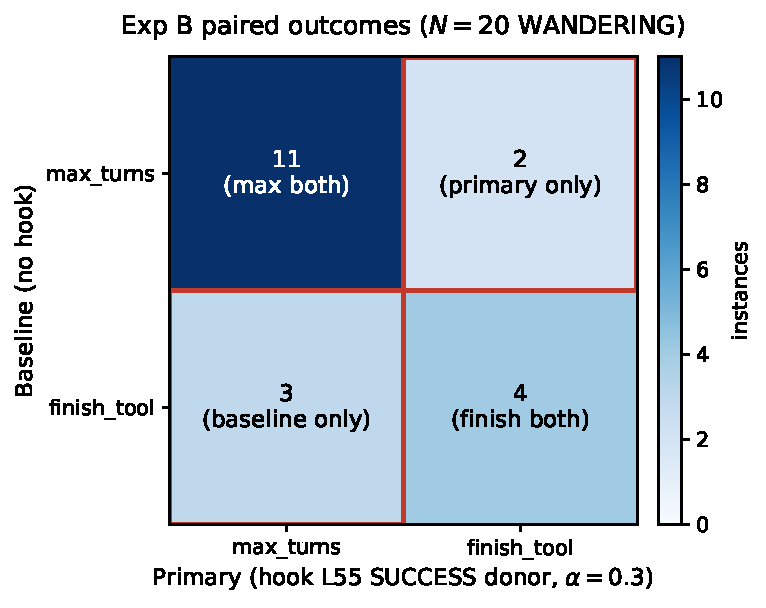
\includegraphics[width=0.75\textwidth]{figures/exp_b_confusion_matrix.pdf}
\caption{Exp B paired confusion matrix. Rows: outcome under Baseline (no hook). Columns: outcome under Primary (hook L55 SUCCESS donor, $\alpha=0.3$). Off-diagonal cells (3 + 2 = 5 discordant pairs) drive the McNemar exact test; the slight asymmetry (3 baseline-only flips vs 2 primary-only flips) is consistent with no causal effect of the hook on \texttt{finish\_tool} emission.}
\label{fig:exp_b_confusion}
\end{figure}

\subsection{Statistical Tests}

\textbf{Fisher's exact} on the 2$\times$2 contingency:
\begin{itemize}
\item Odds ratio: \textbf{0.796} (hook slightly HURT direction)
\item $p$ (two-sided): \textbf{1.000}
\item $p$ (one-sided, primary > baseline): 0.7497
\end{itemize}

\textbf{McNemar's exact} on the discordant-pair structure:
\begin{itemize}
\item Baseline-only flips (hook \emph{blocked} natural finish): 3 instances
\item Primary-only flips (hook \emph{rescued}): 2 instances
\item McNemar exact two-tailed: $p = 1.00$ (binomial CDF saturated at $n_{\text{discordant}}=5$)
\item The slight directional asymmetry --- 3 blocks vs 2 rescues --- favours hook \emph{blocking} natural finishes over \emph{rescuing} WANDERING instances, but the magnitude is well within sampling noise
\end{itemize}

Same outcome in both conditions: 15/20 instances. Eleven max\_turns-in-both, four \texttt{finish\_tool}-in-both. Determinism is largely preserved under same deterministic seed.

\subsection{Per-Instance Paired Comparison}

\begin{table}[h]
\centering
\small
\caption{Exp B --- per-instance paired outcomes. Stars mark instances where conditions disagree.}
\begin{tabular}{lccc}
\toprule
Instance & Baseline & Primary & Changed? \\
\midrule
\texttt{qutebrowser-2dd896} & max\_turns & max\_turns & \\
\texttt{qutebrowser-9b71c1} & finish\_tool & max\_turns & $\star$ baseline only \\
\texttt{openlibrary-5de7de} & finish\_tool & finish\_tool & both \\
\texttt{openlibrary-7f6b722} & max\_turns & finish\_tool & $\star$ primary only \\
\texttt{qutebrowser-0d2afd58} & max\_turns & max\_turns & \\
\texttt{ansible-5d253a13} & max\_turns & max\_turns & \\
\texttt{ansible-502270c8} & finish\_tool & finish\_tool & both \\
\texttt{openlibrary-09865f5f} & max\_turns & max\_turns & \\
\texttt{openlibrary-c05ccf2c} & max\_turns & max\_turns & \\
\texttt{openlibrary-5c6c22f3} & max\_turns & max\_turns & \\
\texttt{openlibrary-bb152d23} & finish\_tool & max\_turns & $\star$ baseline only \\
\texttt{ansible-a26c325b} & max\_turns & max\_turns & \\
\texttt{ansible-3db08adb} & finish\_tool & max\_turns & $\star$ baseline only \\
\texttt{ansible-de01db08} & finish\_tool & finish\_tool & both \\
\texttt{ansible-cd9c4eb5} & finish\_tool & finish\_tool & both \\
\texttt{ansible-4c5ce5a1} & max\_turns & max\_turns & \\
\texttt{qutebrowser-99029144} & max\_turns & max\_turns & \\
\texttt{qutebrowser-85b867fe} & max\_turns & max\_turns & \\
\texttt{qutebrowser-cf06f4e3} & max\_turns & finish\_tool & $\star$ primary only \\
\texttt{qutebrowser-0fc6d110} & max\_turns & max\_turns & \\
\bottomrule
\end{tabular}
\label{tab:exp_b_per_instance}
\end{table}

\subsection{Verdict: Null Causal with Reverse Hint}

The L55 SUCCESS-donor hook at $\alpha=0.3$ produces no statistically significant change in \texttt{finish\_tool} flip rate, and the directional point estimate is slightly negative (hook blocked 3 natural finishes vs rescued 2). The Tool-Entropy mechanism hypothesis, in its simplest form (``persistent SUCCESS-direction at L55 rescues WANDERING''), is refuted at this magnitude.

\subsection{Three Possible Interpretations}

\begin{enumerate}
\item \textbf{Hypothesis correct but L55 isn't the right locus.} Edge-layer alignment failure may involve a different circuit (L11 surface; specific attention heads; MLP-level activations).
\item \textbf{Hypothesis correct but $\alpha=0.3$ too weak.} A structural-rigidity follow-up with $\alpha \in \{0.7, 1.0\}$ would settle this. The reverse-hint direction at $\alpha=0.3$ suggests stronger $\alpha$ may HURT more, not help.
\item \textbf{Hypothesis wrong.} WANDERING may not be ``mid-layer ready, edge fails'' but a fundamentally different mechanism --- for instance, attention-pattern lock-in, or tool-loop reinforcement from in-context examples that no residual-direction perturbation can override.
\end{enumerate}

The \texttt{mode=add} $\alpha=0.3$ experiment was designed to give the hypothesis a fair shot without destroying model coherence (per the \texttt{mode=replace} pivot in \S\ref{sec:exp_b_method}). At this magnitude, the answer is null. The next section tests interpretations 1 and 2 head-on --- the right locus (L11, per the companion paper) across a magnitude sweep --- and finds that fixing both still does not rescue, leaving interpretation 3 standing.

\section{Experiment L11: Edge-Layer Localization with a Norm-Matched $\alpha$-Sweep}\label{sec:exp_l11}

The two leading interpretations of the Exp B null --- wrong locus (L55) and wrong magnitude ($\alpha=0.3$) --- are jointly testable. The companion classification paper \cite{multichannel_2026} provides the locus lead: its stability selection identifies \texttt{L11\_drift\_first\_last} as the dominant WANDERING discriminator (selection frequency $0.95$), surviving an ultra-conservative re-fit, while L55 features do not survive. We therefore re-target the SUCCESS-donor injection to L11 --- WANDERING's strongest \emph{detector} locus --- and ask whether it is also a \emph{lever}.

\subsection{Method}

L11 pre-tool residuals have a much smaller norm than L55 ($\approx 33$ vs.\ $\approx 127$, per-repo SUCCESS-donor means), so the Exp B magnitude ($\alpha=0.3$ at L55) corresponds to $\alpha \approx 1.15$ at L11. We sweep $\alpha \in \{0.35, 0.70, 1.15, 2.30, 4.60\}$ (a single-instance pilot) and then run the full $N=20$ at the two coherence-preserving magnitudes $\{0.70, 1.15\}$, always-on \texttt{mode=add}, per-repo SUCCESS donor. Critically, the comparison is \emph{paired} against the same-session no-hook condition: because WANDERING is not run-stable (\S\ref{sec:run_stability}), the same 20 instances flip \texttt{finish\_tool} $7/20$ with \emph{no} intervention. The only valid test of ``does the hook rescue'' is therefore instance-wise (McNemar), not a comparison against the definitional $0/20$. We additionally run a norm-matched random-direction control --- on the rescued subset only (a selection-biased design we flag below).

\subsection{The robust finding: a dose-dependent destabilization}

\begin{center}
\begin{tabular}{lccc}
\toprule
Condition & \texttt{finish\_tool} & \texttt{max\_turns} & \texttt{invalid\_tools} \\
\midrule
No-hook baseline (paired, \S\ref{sec:run_stability}) & 7/20 (35\%) & 13/20 & 0 \\
L11 hook $\alpha=0.70$ & 5/20 (25\%) & 15/20 & \textbf{0} \\
L11 hook $\alpha=1.15$ & 2/20 (10\%) & 6/20 & \textbf{12/20 (60\%)} \\
\bottomrule
\end{tabular}
\end{center}

The one effect that is unambiguous, large, and not explicable by run-instability is the \texttt{invalid\_tools} column: the L11 hook destabilizes the model into emitting malformed tool calls on $0/20$ runs at $\alpha=0.70$ but $12/20$ ($60\%$) at $\alpha=1.15$. A no-hook re-run never produces \texttt{invalid\_tools}; the single-instance pilot extends the curve ($\alpha \in \{2.30, 4.60\}$ crash at turn 3). This is a clean dose-response and it matters: \textbf{unlike the L55 hook (Exp B), which was behaviorally inert, the L11 hook demonstrably reaches behavior.} The classification paper's locus is causally live. But the direction the perturbation pushes the model is toward \emph{incoherence}, not \emph{completion}.

\subsection{The rescue claim is null --- a walk-back}

A naive reading of the table looks positive: $6/20$ instances flip \texttt{finish\_tool} at one of the two magnitudes, and against the definitional $0/20$ baseline that is Fisher exact $p=0.02$. \textbf{This is the wrong test.} The run-instability finding (\S\ref{sec:run_stability}) shows the correct baseline is the paired no-hook re-run, which flips $7/20$ on its own. Three corrections follow:

\begin{itemize}
\item \textbf{Paired test, $\alpha=0.70$.} Instance-wise, the no-hook baseline flips $7/20$ and the hook flips $5/20$. The discordant pairs are 5 baseline-only (flipped without the hook, suppressed by it) versus 3 hook-only (flipped only with the hook). McNemar exact $p=0.73$ --- \emph{null}, with the point estimate favoring the baseline. The hook does not rescue; if anything it slightly suppresses.
\item \textbf{Contamination of the $6/20$.} Of the six instances that flip at either magnitude, two already flip in the no-hook baseline --- their ``rescue'' is run-instability, not the hook. Only four are clean (no-hook \texttt{max\_turns} $\to$ hook \texttt{finish\_tool}), still fewer than the seven the baseline flips unaided.
\item \textbf{The union framing makes it worse, not better.} Counting ``rescue at either $\alpha$'' gives the intervention two independent draws; the fair baseline (two no-hook draws at $35\%$ each) would itself flip $\approx 12/20$. $6 < 12$.
\end{itemize}

\subsection{Direction-specificity cannot be established here}

The random-direction control was run only on the instances that rescued under the SUCCESS direction (selection on the outcome), and at $\alpha=0.70$ a random direction rescued one of them. Against a $\sim$35\% natural flip rate, ``random rescues $\sim$1 of 5--6'' is exactly what pure instability predicts, so this control cannot distinguish a SUCCESS-direction effect from noise. At $\alpha=1.15$ the random direction \emph{also} crashes the model (\texttt{invalid\_tools}), confirming only that the high-magnitude destabilization is direction-agnostic. A direction-specificity claim would require running both SUCCESS and random directions on all 20 instances; we did not, and we make no such claim.

\subsection{Verdict: The Right Locus, but Not a Rescue Lever}

L11 is where WANDERING is most legible (companion paper \cite{multichannel_2026}) and the L11 SUCCESS-donor hook is demonstrably causal (dose-dependent destabilization). But on the question this experiment was built to answer --- does injecting the SUCCESS edge-direction \emph{rescue} WANDERING --- the answer is null (paired McNemar $p=0.73$), the third null in this paper. Correcting the locus from L55 to L11 did \emph{not} close the gap between detection and intervention; it relocated the failure from ``inert'' to ``live but un-steerable-to-finish''. The companion paper independently shows that \emph{which} agents flip is predicted by tool-entropy collapse depth, not by the residual signature --- consistent with the lever, if one exists, not being a static residual direction at all.

\section{Methodological Discovery: WANDERING Is Not Run-Stable}\label{sec:run_stability}

The Tool-Entropy paper trained Phase 6 on an NVIDIA RTX 6000 Pro Blackwell (96 GB) and classified all 20 of the trajectories considered here as \texttt{max\_turns} (0/20 \texttt{finish\_tool}). That classification is, by construction, what defines them as WANDERING.

When we re-ran the same 20 trajectories on RTX 6000 Pro Blackwell 96\,GB with the same deterministic seed (\texttt{Runner.seed\_for(iid)}) and no hook installed (the Exp B Baseline condition), 7 of the 20 (35\%) emitted \texttt{finish\_tool}; a fresh same-session determinism check yielded 0/5. The classification did not reproduce run-to-run on identical hardware.

\textbf{What is happening.} Generation uses sampling at temperature 1.0, which is not bit-reproducible run-to-run even with a fixed nominal seed (kernel/batch nondeterminism plus library-version drift). Small numerical differences in attention/MLP cascades drift the model into different action choices over 50 turns, and seven of twenty WANDERING-labelled trajectories happen to choose \texttt{finish\_tool} on an independent re-run where they did not in the original Phase 6 run --- on the same RTX 6000 Pro Blackwell hardware.

\textbf{Implications.}
\begin{itemize}
\item The WANDERING phenotype as captured by single-run classification is at minimum a 35\% run-to-run noise floor under temperature sampling --- i.e., a substantial fraction of WANDERING is sampling-stochasticity artifact, not robust behavioral mode.
\item It is tempting to restrict analysis to the $13/20$ that exhaust in \emph{both} the original run and the no-hook re-run --- a ``stable WANDERING'' subset --- and report the hook flip rate there against a $0/13$ baseline. We flag this as a \emph{trap}, not a result: conditioning on the baseline being \texttt{max\_turns} selects exactly the instances where any subsequent flip (caused by the hook or by nothing) reads as a rescue, and at a $\sim$35\% instability floor a hook that does nothing would still flip $\sim$3--4 of 13 against that rigged $0/13$. This is the same wrong-baseline error as the naive Fisher in \S\ref{sec:exp_l11}. The honest comparison stays paired and unconditioned, and it is null.
\item Future WANDERING labelling protocols should require multi-seed classification at a single GPU (run $k$ times with seeds $\{0, \ldots, k-1\}$, classify as WANDERING only if all $k$ exhaust the budget).
\end{itemize}

This finding does not invalidate the Tool-Entropy paper's substantive contributions (cross-architecture generalization of the entropy signature, scope-limited cross-task validation). It does refine the WANDERING category itself: $\sim$35\% of what was labelled WANDERING is run-to-run stochasticity artifact under temperature$=$1.0 re-run.

\section{What Does This Mean for the Tool-Entropy Mechanism Hypothesis?}\label{sec:mechanism_implications}

Three causal tests, read together, refute the \emph{actionable} form of the Tool-Entropy \S13 hypothesis while leaving its descriptive form untested:

\begin{itemize}
\item ``WANDERING agents knew the answer'' is not supported (Exp D): forced-finish patches do not pass at a different rate.
\item ``Persistent SUCCESS \emph{L55} direction injection rescues WANDERING'' is not supported (Exp B): the hook is behaviorally inert.
\item ``Persistent SUCCESS \emph{L11} direction injection rescues WANDERING'' is not supported (Exp L11): paired McNemar $p=0.73$. The L11 hook is causally live (dose-dependent destabilization) but pushes toward \texttt{invalid\_tools}, not \texttt{finish\_tool}.
\end{itemize}

The \S13 hypothesis has a descriptive claim (``mid-layer verdict consolidated; edge circuits fail to translate it into the finish action'') and an actionable corollary (``so injecting the SUCCESS edge-direction should supply the missing translation and rescue''). This paper tests the corollary three ways and falsifies it three times. The descriptive claim is neither confirmed nor denied --- we never read the mid-layer verdict directly, and a failed injection is consistent with both ``the verdict was never really consolidated'' and ``the verdict is consolidated but the edge computation is not a linearly-addable direction''. Our data slightly favor the latter: L11 injection clearly perturbs the edge computation (it can break it), it just cannot be steered to the finish action.

The crucial negative is about \emph{locus}. The companion classification paper \cite{multichannel_2026} identifies L11 --- not L55 --- as WANDERING's strongest discriminator by stability selection (selection frequency $0.95$; L55 features do not survive). One might expect that intervening at the \emph{right} layer would convert the L55 null into a positive. It does not. Correcting the locus moved the result from ``inert'' (L55) to ``live but un-steerable-to-finish'' (L11), but not to ``rescue''. The detection/intervention gap is therefore not a locus error that triangulation can close.

What remains genuinely open:
\begin{itemize}
\item Whether a \emph{non-linear} or \emph{transient} edge intervention (a pulse fired at the lock-in turn, rather than an always-on additive direction) could rescue. The inverted-U (\S\ref{sec:exp_l11}) shows the additive direction has only a destabilizing regime above threshold and a null regime below it; a different intervention class is untested.
\item \emph{Which} agents are even candidate-rescuable is predicted by tool-entropy collapse depth (\cite{multichannel_2026}, Phase 6: AUC $0.77$, $p=0.07$) and \emph{not} by the residual signature (4-feature LOO-AUC $0.62$, $p=0.16$, fails its gate). If a lever exists, the evidence points to it being indexed by behavior, not by a static residual direction.
\end{itemize}

The v5 tool-entropy signal remains a useful \emph{detector} (correlative): WANDERING agents reliably show entropy collapse in the last 10 turns relative to SUCCESS, generalizing cross-architecture. What all three experiments refute is the move from detector to one-shot residual \emph{lever} --- at L55 (inert), and, more tellingly, at L11, the very locus that detects WANDERING best. Detection does not imply a steerable direction, even at the strongest locus. This sharpens the correlative-vs-causal distinction the ``Two Forms of Epiphenomenal Probes'' line \cite{two_forms_2026} formalized: the gap between a detector and a lever is not always a gap in \emph{locus} that better targeting can close.

\section{Joins the Pattern of Epiphenomenal Detectors}

Across three prior null results from the same research program (Phase 7: softmax-temperature epiphenomenon for L43 \texttt{pre\_tool} probes; Phase 8: template-locked epiphenomenon for L55 \texttt{think\_start} probes; \cite{two_forms_2026}) and this paper (Exp B null for L55, and Exp L11 null-on-rescue at L11, both SUCCESS-donor injection), a stable pattern emerges:

\begin{quote}
\textit{Predictive signals in residual streams are routinely correlative without being causal. Discovering a signal that distinguishes failure from success does not imply that intervening on that signal direction will alter behavior.}
\end{quote}

The mechanism by which signals become epiphenomenal varies --- softmax-temperature confound (Phase 7), template-locked output structure (Phase 8), an edge-direction that detects WANDERING but cannot steer it to completion (this paper). In each case, the corrective is the same: \emph{causal tests with proper controls, before deploying correlative signals as steering levers}.

Exp L11 sharpens the pattern rather than excepting it. One natural rescue for an epiphenomenal-detector result is ``we targeted the wrong layer''; triangulating to the right locus should then convert the null. We ran exactly that test --- the companion paper's stability selection hands us L11 as WANDERING's strongest discriminator --- and the rescue intervention is still null there (paired McNemar $p=0.73$). The signal is correlative \emph{even at its strongest locus}. That is a stronger statement than ``wrong layer'': the detector/lever gap here is not a targeting error.

For Tier 3 autonomous-termination signals (using v5 entropy as a probe-free hard escalation), this does not undermine deployment: the detector still works correlatively at the precision-recall reported in Tool-Entropy. What it forecloses is the temptation to flip the same signal into a one-shot rescue intervention: injecting the SUCCESS direction does not rescue at L55 (inert) or at L11 (live but destabilizing). A detector is not a free intervention --- and, here, not an intervention at all.

\section{Limitations}\label{sec:limitations}

\textbf{Sample size.} $N=20$ WANDERING for Exp B yields modest statistical power. A 30 pp effect requires $\sim$17 discordant pairs at $\alpha=0.05$, $\beta=0.20$ for McNemar's exact; we observed 5 discordant pairs (3 vs 2), which would not be significant even if all were in the same direction.

\textbf{Single magnitude tested at L55.} Only $\alpha=0.3$ was run for Exp B at L55. Exp L11 addresses magnitude at L11 (five-point sweep), but L55 was never re-swept; we cannot exclude that L55 has its own usable band at some untested magnitude. The L11 result makes this less interesting (L11 is the locus the companion paper points to), not moot.

\textbf{L11 null --- power, and what is \emph{not} power-limited.} The paired McNemar for L11 rescue ($p=0.73$) is a null, not a demonstrated absence of any effect: with 8 discordant pairs the test could only have caught a large rescue, so a small genuine rescue cannot be excluded. The point estimate, however, favors the baseline, and the union/contamination corrections (\S\ref{sec:exp_l11}) all push the same way. What is \emph{not} power-limited is the dose-dependent destabilization ($0/20 \to 12/20$ \texttt{invalid\_tools}), which is large and unambiguous. The random-direction control was run only on the rescued subset ($n=5$, selection-biased) and cannot establish direction-specificity in either direction; a full-$N$ SUCCESS-vs-random arm is needed (\S\ref{sec:future_work}).

\textbf{Single intervention type.} Plan B (always-on hook) was chosen over Plan A (transient surgical patch at lock-in turn) because of trajectory-replay determinism risk (only 5/20 trajectories met the $\geq$80\% replayable criterion). Plan A remains a legitimate alternative test of a slightly different prediction.

\textbf{Single hardware for the experiments themselves.} Exp D, Exp B, and Exp L11 all ran on RTX 6000 Pro Blackwell 96\,GB. We have not tested whether the nulls reproduce on a different GPU class --- though, given run-instability is the central methodological finding, the relevant variation is across seeds, not hardware.

\textbf{Probe-derived direction not tested.} All three injection tests used a SUCCESS \emph{donor} direction. A different causal test (\S\ref{sec:future_work}, ``Exp C'') would use the v5 collapse direction at L43 with an $\alpha$-sweep and random-direction control. We already have three nulls (Exp D, L55, L11); a fourth, with a probe-derived rather than donor direction, would further constrain whether \emph{any} static residual direction is a WANDERING lever.

\section{Future Work}\label{sec:future_work}

\textbf{Full-$N$ direction-specificity arm}: run SUCCESS-donor and norm-matched random-direction injection on all 20 instances at $\alpha=0.70$ (not just the rescued subset), so the SUCCESS-vs-random contrast is unbiased. This is the clean test of whether the (null-on-average) L11 effect hides any direction-specific component the paired test could not resolve at $N=20$. $\sim$8 h on RTX 6000 Pro Blackwell, $\sim$\$16 \texttt{vast.ai}.

\textbf{Transient L11 pulse (v5-gated closed loop)}: the always-on additive direction has only a null regime (low $\alpha$) and a destabilizing regime (high $\alpha$), with no rescue regime (\S\ref{sec:exp_l11}). A different intervention \emph{class} --- a transient pulse fired only at the tool-entropy collapse turn, rather than an always-on direction --- is untested and is the most informative next experiment. Crucially, the gate should be the v5 tool-entropy signal, \emph{not} the residual signature, because candidate-rescuability is behavior-legible and residual-blind (\cite{multichannel_2026}, Phase 6).

\textbf{Plan A (transient surgical patch at lock-in turn)}: engineering-heavier but tests a different prediction. Requires either deterministic trajectory replay (5/20 replayable) or sandbox state injection.

\textbf{Exp C (v5 collapse direction $\alpha$-sweep at L43)}: tests a different direction (probe-derived, not SUCCESS donor) at a different layer (L43 mid vs L55 edge). Designed with random-direction control and structural-rigidity diagnostic. $\sim$8 h, $\sim$\$16.

\textbf{Multi-seed WANDERING classification protocol}: re-run all Phase 6 trajectories $k$ times at single hardware with different seeds; classify as WANDERING only when all $k$ exhaust budget. Provides run-stable labels for future causal work.

\textbf{Pre-registered run-stable labels}: rather than the post-hoc ``stable subset'' trap (\S\ref{sec:run_stability}), re-run all Phase 6 trajectories $k$ times \emph{up front}, define WANDERING only on instances that exhaust on all $k$ seeds, and \emph{then} run a fresh paired intervention on those pre-registered labels. This is the only way to ask the stable-subset question without conditioning on the baseline outcome.

\section{Conclusion}

We report three causal tests of the Tool-Entropy WANDERING mechanism hypothesis (``mid-layer verdict consolidated, edge-layer alignment fails''), and all three are null on the question of \emph{rescuing} WANDERING. The Exp D forced-finish counterfactual rules out ``silent success'': WANDERING patches do not pass tests at a different rate than SUCCESS patches (Fisher $p=0.71$). The Exp B always-on \emph{L55} SUCCESS-donor steering is behaviorally inert (Fisher $p=1.00$). Re-targeting the same intervention to \emph{L11} --- the edge layer that the companion classification paper \cite{multichannel_2026} independently flags as WANDERING's strongest discriminator --- and sweeping magnitude does \emph{not} rescue either (paired McNemar $p=0.73$); a naive Fisher test against the definitional $0/20$ baseline reads $p=0.02$, but that baseline is invalidated by run-instability and the paired test is null.

The one robust causal effect we find is the opposite of a rescue: at higher magnitude the L11 hook destabilizes the model into \texttt{invalid\_tools} on $12/20$ runs ($0/20$ at the lower magnitude; $0/20$ with no hook). L11 injection plainly \emph{reaches} behavior --- unlike the inert L55 hook --- but pushes toward incoherence, not completion.

We additionally surface a load-bearing methodological finding: the WANDERING classification is not run-stable under temperature$=$1.0. Same-seed independent re-runs (same RTX 6000 Pro Blackwell hardware) of trajectories labelled WANDERING emit \texttt{finish\_tool} up to 35\% of the time. This is why every intervention test must be paired, and why the unpaired $0/20$ comparison manufactures a false positive.

The arc --- detector (Tool-Entropy v5) $\to$ inert at L55 $\to$ live-but-un-steerable at L11, the strongest detector locus --- is the paper's contribution. Correcting the locus did not convert the null: the SUCCESS direction detects WANDERING without being a lever to fix it, \emph{even at the layer where detection is strongest}. The Tool-Entropy v5 detector remains useful for forensics, advisory escalation, and Tier 3 autonomous termination at its reported precision-recall; the move from that detector to a one-shot residual rescue is, at both edge layers tested, false. Where a lever might still live --- a transient, behavior-gated intervention rather than an always-on residual direction --- is the next paper's question.

\section*{Data and code availability}
All code --- the always-on steering hook, the L11 $\alpha$-sweep, the paired McNemar analysis (\texttt{scripts/paper2\_l11\_honest\_paired\_analysis.py}), the Exp D Docker patch-pass harness, and the figure generators --- is released under Apache-2.0 at \url{https://github.com/OpenInterpretability/openinterp-swebench-harness}. The underlying Phase-6 trajectories and residuals are on HuggingFace at \texttt{huggingface.co/datasets/caiovicentino1/swebench-pro-qwen36-27b-phase6}. Companion paper: Tool-Entropy Collapse (DOI~\texttt{10.5281/zenodo.20368601}).

\bibliographystyle{plain}
\bibliography{references}

\appendix

\section{Appendix A: Exp D Per-Instance WANDERING Verdicts}\label{app:exp_d_per_instance}

Table \ref{tab:exp_d_wandering_full} lists all 19 Docker-evaluated WANDERING trajectories with their \texttt{agent} condition pass/fail breakdown.

\begin{table}[h]
\centering
\small
\caption{Exp D --- all WANDERING agent-patch verdicts.}
\begin{tabular}{llrrr}
\toprule
Instance & Verdict & \texttt{n\_pass} & \texttt{n\_fail} & \texttt{n\_err} \\
\midrule
\texttt{qutebrowser-2dd896} & FAIL & 0 & 0 & 0 \\
\texttt{qutebrowser-9b71c1} & FAIL & 0 & 0 & 0 \\
\texttt{openlibrary-5de7de} & FAIL & 9 & 16 & 0 \\
\texttt{openlibrary-7f6b722} & FAIL & 5 & 0 & 2 \\
\texttt{openlibrary-09865f5f} & FAIL & 12 & 1 & 0 \\
\texttt{openlibrary-5c6c22f3} & FAIL & 20 & 2 & 0 \\
\texttt{openlibrary-bb152d23} & FAIL & 0 & 3 & 0 \\
\texttt{ansible-3db08adb} & FAIL & 47 & 2 & 0 \\
\texttt{ansible-de01db08} & FAIL & 3 & 1 & 0 \\
\texttt{ansible-cd9c4eb5} & FAIL & 0 & 1 & 0 \\
\texttt{ansible-4c5ce5a1} & FAIL & 8 & 9 & 4 \\
\texttt{qutebrowser-99029144} & FAIL & 12 & 2 & 0 \\
\texttt{qutebrowser-85b867fe} & FAIL & 266 & 11 & 0 \\
\texttt{qutebrowser-cf06f4e3} & FAIL & 30 & 10 & 10 \\
\texttt{qutebrowser-0fc6d110} & FAIL & 0 & 0 & 0 \\
\texttt{qutebrowser-0d2afd58} & PASS & 66 & 0 & 0 \\
\texttt{ansible-502270c8} & PASS & 1 & 0 & 0 \\
\texttt{openlibrary-c05ccf2c} & PASS & 95 & 0 & 0 \\
\texttt{ansible-a26c325b} & PASS & 42 & 0 & 0 \\
\bottomrule
\end{tabular}
\label{tab:exp_d_wandering_full}
\end{table}

\section{Appendix B: Exp B Plan B Implementation Details}\label{app:exp_b_implementation}

The \texttt{LayerPatch} class installs a forward hook on \texttt{model.model.layers[L]} that modifies the residual stream output at the last token position:

\begin{verbatim}
def hook(module, inputs, output):
    hs = output[0] if isinstance(output, tuple) else output
    patch = patch_tensor.to(device=hs.device, dtype=hs.dtype)
    with torch.no_grad():
        if mode == 'add':
            hs[0, -1, :] = hs[0, -1, :] + alpha * patch
        elif mode == 'replace':
            hs[0, -1, :] = patch
    return (hs,) + rest if rest else hs
\end{verbatim}

The hook fires on every forward pass through L55 --- both during prefill (once per input position) and during autoregressive decode (once per generated token). For a typical 50-turn WANDERING run, the hook is called $\sim$10{,}000-25{,}000 times.

\textbf{Sanity check}: hook call count per instance ranged from 6{,}397 to 64{,}172 in the Primary condition, scaling with total tokens generated. The Baseline runs (no hook) have zero hook calls by construction. VRAM peak ranged 57.7-72.1 GB across conditions, well under the RTX 6000 Pro Blackwell 96 GB ceiling.

\section{Appendix C: Compute Budget}

\begin{table}[h]
\centering
\small
\caption{Compute consumed for paper \#2 experiments. All GPU runs used one RTX 6000 Pro Blackwell 96\,GB on \texttt{vast.ai}; Exp D ran on a local Mac CPU. Exp L11 wall times are estimated by analogy to the measured Exp B run (the L11 session was executed without a saved timing log); the Exp L11 \emph{outcomes} are exact (per-instance \texttt{finish\_tool}/\texttt{max\_turns} verdicts, \S\ref{sec:exp_l11}).}
\begin{tabular}{lr}
\toprule
Experiment & Wall time \\
\midrule
Exp D (Phase 6b Docker eval, local Mac CPU) & $\sim$10 min \\
Exp B Primary (20 WANDERING, L55 hook) & 395 min \\
Exp B Baseline (20 WANDERING, no hook) & 374 min \\
Exp L11 pilot ($\alpha$-sweep, 1 instance $\times$ 5) & $\sim$25 min (est.) \\
Exp L11 Phase 1 (20 WANDERING $\times$ 2 $\alpha$) & $\sim$790 min (est.) \\
Exp L11 random-direction control (5 instances) & $\sim$100 min (est.) \\
\bottomrule
\end{tabular}
\end{table}

Total GPU compute (RTX 6000 Pro Blackwell) on \texttt{vast.ai} at $\sim$\$1.50--2/h: $\sim$\$50 (Exp B $\sim$\$20 measured; Exp L11 $\sim$\$30 estimated).

\section{Appendix D: Methodological Heritage from Prior Work}

The Plan A vs Plan B design discussion was informed by the trajectory-replay determinism audit (\texttt{scripts/exp\_b\_determinism\_check.py}): only 5/20 WANDERING trajectories had $\geq 80\%$ replayable tool-calls (the rest contained \texttt{pip}/\texttt{pytest}/\texttt{python}/\texttt{git} commands with non-deterministic outputs), motivating the pivot to Plan B always-on hook.

The \texttt{mode=replace} $\rightarrow$ \texttt{mode=add} pivot was forced by the initial \texttt{mode=replace} attempt producing \texttt{invalid\_tools} parser errors within 3 turns on every instance. The mechanism is mechanical: substituting L55 residual with a constant donor every forward pass forces L56-L63 to read identical input on every new decode token, destroying contextual generation. The fix is to use additive steering (preserves residual variation while injecting a persistent bias) rather than substitutive patching. This pivot is recorded in our memory of practice as \texttt{feedback\_always\_on\_replace\_destructive}.

\end{document}
